\chapter{Evaluation}
\label{cha:evaluation}

In this chapter, we present the first set of results and insights drawn from our NTT architecture. We begin with an overview of the data and setup for evaluation, followed by an initial evaluation and use the results from this,  to draw further insights and carry out further, more robust evaluation.

\section{Initial Evaluation Setup}
\label{eval:evaldat}

We have already discussed in detail the dataset used for pre-training in Section \ref{sec:ns3} and the objectives in Section \ref{ssec:despatt}. For testing the initial performance of our pre-training process, we reserve a random $10\%$ of the sequences from our pre-training data. This data is always used just for testing, the model does not see this data during the pre-training phase ever, and the testing dataset is always the same across any kind of comparing experiment.

\begin{figure}[h]
  \begin{center}
    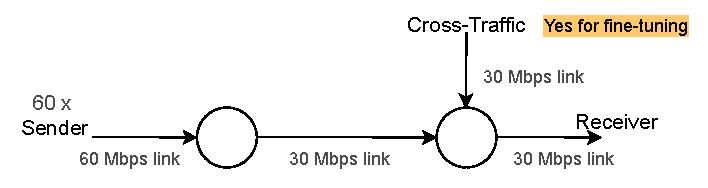
\includegraphics[scale=1.2]{figures/simple_topo_ft.pdf}
    \caption{Fine-tuning data generation}
    \label{fig:topo_ft}
  \end{center}
\end{figure}

The setup for the fine-tuning dataset is the same, except that we add a second bottleneck for sender traffic by introducing $20$ Mbps of TCP cross-traffic on the rightmost link. The dataset does \emph{not} explicitly contain the cross-traffic; we \emph{only} collect packets from the senders. However, the introduction of this cross traffic affects the dynamics of the overall network due to  congestion, which in turn affects the dynamics in the behaviour of the applications sending traffic. We demonstrate this setup in Figure \ref{fig:topo_ft}. For our initial evaluation, we generate one simulation run of fine-tuning data only and this dataset contains about 115 thousand packets, \ie roughly $1/10$\textsuperscript{th} of the pre-training dataset. To ensure our training is not affected by extremely large possible ranges of values, we normalise our input features of size and delay, over the mean and standard deviation of each feature over the entire data, individually.\cite{scaling} Based on the fine-tuning dataset generated, we have two fine-tuning tasks 

\begin{itemize}
\item \emph{Fine-tuning on new environment:} In this fine-tuning task, we try to predict the last delay in the sequence, on data generated on a new topology with $2$ bottlenecks, as opposed to pre-training where we had $1$ bottleneck. Our pre-training process employs multiple kinds of masking over different delay positions, but for the fine-tuning task objective is prediction of the delay at the last position. The \emph{key idea} is to use the learn sequence structure in the during the pre-training and apply it to predict the last delay and make a decision on the final packet during the fine-tuning, following a change in network environment. We expect that if the pre-training is done robustly, fine-tuning in this new environment on a similar task will be both faster and require significantly less data.

\item \emph{Fine-tuning on a new task:} In this fine-tuning task, we try to predict the Message Completion Time (MCT) of an entire transmitted message, given the NTT's encoded output states of the previous $1024$ packets and the size of the given message. Our fine-tuning objective is to mean pool\cite{poolcv}\cite{zaheerDeepSets2018} over all the NTT's output states which represents the overall learnt behaviour of the network dynamics in the recent past. We combine this learnt feature with the message size, which we can have in our simulation data using appropriate features from our Network Simulator\cite{ns3} and use this to predict the MCT using a Multilayer Perceptron with linear layers. The \emph{key idea} is to learn the \emph{overall} structure from the network dynamics and use it to predict tasks, which depend on the nature of these dynamics.
\end{itemize}

For evalaution, we calculate the mean-squared error (MSE) for achieved on both tasks and report our initial findings in Table \ref{eval:table1}. We process MCTs on a logarithmic scale to limit the impact of outliers. This is required as our MCT dataset is quite heavy tailed, which hurts training deep learning models.\footnote{Our simulation's mean and 99.9th percentile MCTs are 0.2 and 23 seconds, respectively.}


\section{Preliminary Results}
\label{eval:pres}

In our initial experiments, we compare several versions of our NTT, vary both our pre-training and fine-tuning objectives, in order to explore the possibilities of what information can actually be learnt and to which extent. We focus on evaluating and demonstrating on the following points:

\begin{itemize}
\item Our NTT is capable of learning network dynamics from packet data 
\item Pre-training enables our NTT to generalize on new environments and new tasks 
\item Incorporating our networking domain specific knowledge helps the NTT perform better
\end{itemize}

We demonstrate our initial comparison in Table \ref{eval:table1} The \emph{pre-trained} model first learns from the pre-training and then from the fine-tuning dataset, while the \emph{from scratch} version only learns from the fine-tuning dataset. In these experiments, the fine-tuning dataset is only around $1/10$\textsuperscript{th} of the size of the pre-training dataset. In all the NTT variants presented here, we only mask the last packet delay during the pre-training process.\footnote{Further details on training (\eg hyperparameters) have been moved to the Appendix \ref{app:a}.}

In order to evaluate the choice of our feature selection for pre-training , we perform some ablation studies on the input data. We argue that we need both packet state information and network state information to effectively learn network dynamics. In order to investigate this, we pre-train two additional versions of the NTT, one \emph{without delay} and one \emph{without packet size} information, in the respective input sequences. For both our pre-training and fine-tuning, we reserve a part of the datasets for testing, which is always constant, unknown to the model and same across every NTT variant.

We also perform ablation studies to investigate the effects of aggregating features in our input, which we feed into the encoder stage of our NTT. Concretely, we compare our multi-step aggregation of $1024$ packets into $48$ aggregates (see Section \ref{ssec:desagg}) with \emph{no aggregation} (using only $48$ individual packets) and \emph{fixed aggregation} (using $48 $ aggregates of $21$ packets each, \ie $1008$ packet sequences). Due to limits of our training infrastructure and Transformer's quadratic scaling behaviour with increasing sequence size, it is infeasible to evaluate the effects of having no aggregation on very large sequences.



\begin{table}[htbp]
\centering
\begin{tabular}{ l   c   c  c }
\toprule
\emph{all values $\times10^{-3}$} & Pre-training  & \multicolumn{2}{c}{Fine-tuning} \\
\cmidrule{3-4}
                                                       & {Delay}        & {Delay}                           & {log MCT} \\
\midrule
\em{NTT}                                                 &                &                                   &           \\
    \smallindent Pre-trained                                 & 0.072          & 0.097                             & 65        \\
    \smallindent From scratch                                & {-}            & 0.313                             & 117       \\
    \noalign{\vskip 1mm}
    \em{Baselines}                                                                                                                 \\
    \smallindent ARMA                                            & 1.800        &  1.180                              &1412 \\
    \smallindent Last observed                               & 0.142          & 0.121                             & 2189      \\
    \smallindent EWMA                                        & 0.259          & 0.211                             & 1147      \\
    \noalign{\vskip 1mm}
    \em{NTT (Ablated)}                                                                                                        \\
    \smallindent No aggregation                              & 0.258          & 0.430                             & 61        \\
    \smallindent Fixed aggregation                           & 0.055          & 0.134                             & 115       \\[0.75mm]

    \smallindent Without packet size                         & 0.001          & 8.688                             & 94        \\
    \smallindent Without delay                               & 15.797         & 10.898                            & 802       \\
     \bottomrule

\end{tabular}
\caption{Mean Squared Error for all initial NTT models and tasks. The MSE is computed on the task specific actual value vs the predicted value of the particular model. The MSE is always calculated on the same test dataset.}
\label{eval:table1}
\end{table}

We also to ensure that we understand if our NTT learns useful information in the first place. To put this into perspective, we use the following three simple baselines in order to compare the performance of our different NTT variants. 
\begin{itemize}
\item \emph{Auto-Regressive Moving Average (ARMA)\cite{arma}:} In this method, we predict the mean delay of all the previous delay values in our sequence as our target delay value.
\item \emph{Last observed:} In this method, we predict the last observed delay over all the previous delay values in our sequence as our target delay value.
\item \emph{Exponentially Weighted Moving Average (EWMA)\cite{ewma}:}  In this method, we predict a weighted smoothed mean delay of all the previous delay values in our sequence as our target delay value.\footnote{For our EWMA, we use the decay factor $\alpha=0.01$} 
\end{itemize}

\paragraph*{NTT can learn some network dynamics:}

Based on the initial evaluation, we confirm that the \emph{pre-trained} NTT beats our baselines in all cases. Though the baselines are rather basic, we can already conclude that the NTT learns the network dynamics to an extent and that the 
the error values are sensible. We also observe that some of the baselines work reasonably, depending on the complexity of the task. For \eg the smoothed \emph{EWMA} approach works reasonably well for delay prediction, it fails for the more complex MCT task.
On the delay task, we further observe that the \emph{last observed} baseline performs better than \emph{EWMA}; that is, smoothing over a long sequence performs worse than simply returning the most recent packet.
This suggests that there is something to learn from the \emph{sequence dynamics}, which the NTT can do much better, as we see it perform better for both types of fine-tuning tasks. This suggests that the NTT can learn fine-grained sequence information, along with aggregated structural information from the entire sequence.

\begin{figure*}[!h]
  \begin{center}
    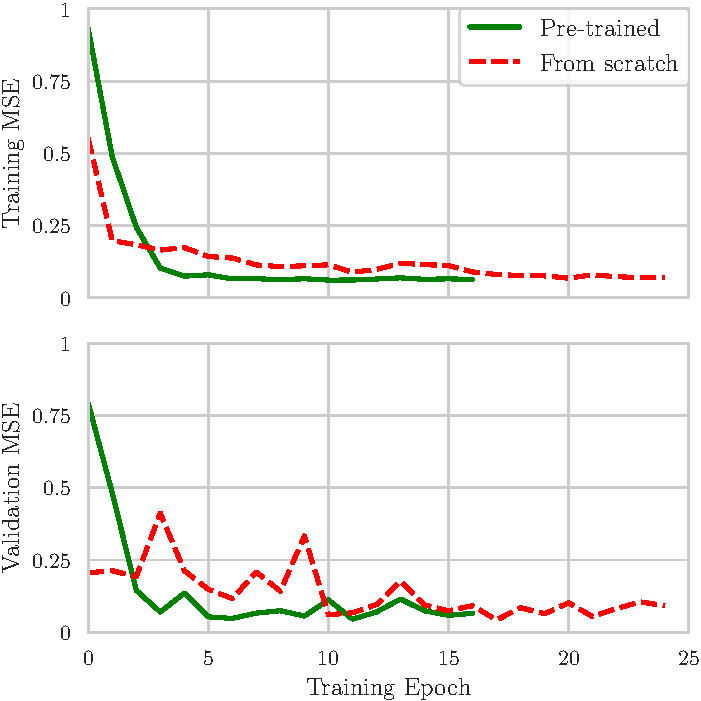
\includegraphics[scale=1]{figures/MCT_loss.pdf}
    \caption{Mean-square error for prediction of message
time completion over training epochs}
    \label{fig:loss_mct}
  \end{center}
\end{figure*}

\vspace{-1cm}

\paragraph*{NTT can generalize across environments and tasks:}

We observe that pre-training is beneficial: on both fine-tuning tasks, the \emph{pre-trained} NTT outperforms the \emph{from scratch} version.The pre-training knowledge generalizes to a new environment \ie unobserved cross-traffic and to a new task \ie MCT prediction. In our current NTT variants, we pre-train and fine-tuning for delay prediction in the exact same way, by learning to predict the last delay in the sequence. Pre-training also improves the speed of the fine-tuning process, in addition to the overall performance. We see this in Figure \ref{fig:loss_mct} shows that pre-training allows faster learning on the fine-tuning dataset: the \emph{pre-trained} NTT reaches a lower error after a few (only 3) training epochs and finishes training, \ie no further improvement, after fewer epochs (17 vs 25), with a lower MSE on the test set in the end (Table \ref{eval:table1})


\paragraph*{NTT specific features help:}
Finally, we argue about about the benefits of the two NTT-specific features we propose: \ie the hierarchical aggregation layer and the mix of network and traffic information in the raw data.

With \emph{no aggregation}, the model has little history available; we observe that, perhaps surprisingly, this affects the predictions on the delay, but not on the MCT. Conversely, with a \emph{fixed aggregation}, the model loses recent packet-level details but has access to longer history; this seems sufficient to predict delays but affects the MCT.\footnote{In the vision transformer\cite{dosovitskiyImageWorth16x162021}, they got extremely good results with fixed size aggregations and very large training datasets.}
It is a little early to map the exactness of these effects at this point, however we can conclude from this initial result suggests that both recent packet level information and longer historical aggregates are useful to generalize to a large set of tasks.


Considering the NTT versions \emph{without packet size} and \emph{without delay} information (Table \ref{eval:table1}), we observe that neither generalize well.
Without the packet size, the model overfits the pre-training dataset and performs poorly on predicting delay for fine-tuning. This is not surprising as given only a single feature, the model cannot learn relational information well.
Without delay information, the model does not produce any useful prediction related to packet delays or MCTs. This is also not surprising as we cannot expect to predict any useful information about the network dynamics, without using any data from it.


Based on the promising nature of our initial results, we now move to more robust evaluation, harder and more generic pre-training and fine-tuning objectives, in order to explore to what further extent can our NTT perform. We explore further methods to analyse and improve our NTT in the following Section \ref{eval:fres}


\section{Further Results}
\label{eval:fres}

\subsection{NTT vs improved baselines}
\label{ssec:impbase}

Our initial experiments show that our NTT learns sequence structure from the packet data reasonably well, and we have several baselines to argue that we learn useful information. Since our initial baselines are rather simple, we now present further analysis against more improved and tuned-baselines, in order to understand the learning behaviour of our NTT better. Our objective of using these new baselines is \emph{NOT} to show that our NTT outperforms them by significant order (given that we work in a small setup with limited data), but rather to put into perspective the nature and complexity of learning the sequence structure of our in general. We argue that learning structure from our data is not trivial, even across a variety of models which learn structural information in very different ways.

\paragraph*{Auto Regressive Integrated Moving Average:}

We first present an Auto Regressive Integrated Moving Average (ARIMA)\cite{arima} model as a method to learn structure in the data. As the ARIMA algorithm is capable of only learning from a single time-series of real numbers, we present it the past history of \emph{delay values}, and fit the model on these values, in order to predict the subsequent delay value. Our choice of this model as a baseline is due to the fact that the ARIMA  model has successfully been used in several types of time-series forecasting\cite{arimasuc}. We have a \emph{one-step rolling} ARIMA forecast, where at every stage, we fit the entire history of all previous delay values to predict the next delay, following which we shift our window forward by $1$, and carry out the same procedure. We carry out the ARIMA rolling forecast over the delay values from our pre-training dataset (see Section \ref{sec:ns3}) and keep the minimum past history size of $1023$ values, in order to have enough past values and also in conjunction with our bottleneck queue size, as we did for the NTT's sequence definition.

We refer to the learnt behaviour by fitting ARIMA in Figure \ref{fig:arima} and present two models, one with increasing history size up to the previous $10000$ and another with upto $30000$ past delay values. It is evident that the squared errors in the ARIMA models do not stabilise even after fitting on increasing past history sizes. This shows that the structure in our packet data cannot be trivially learnt by just fitting on previous values, we need some features which help understand the network dynamics, and this is the very problem we try to solve using our NTT. Even in terms of efficiency, the one step rolling forecast ARIMA model on increasing history size, doesn't scale. We require a fitting time of ${\sim}1.5$ hours for a past history window size upto $10000$ and ${\sim}13$ hours for a past history window size of $30000$, which also practically limits us from fitting much larger windows. In similar time orders to fitting on upto the $30000$ past history, our NTT learns network dynamics to a significant extent and is able to generalize to new tasks (demonstrated in Table \ref{eval:table1}).

\begin{figure*}[h]
    \centering
    \begin{subfigure}[h]{0.5\textwidth}
        \centering
        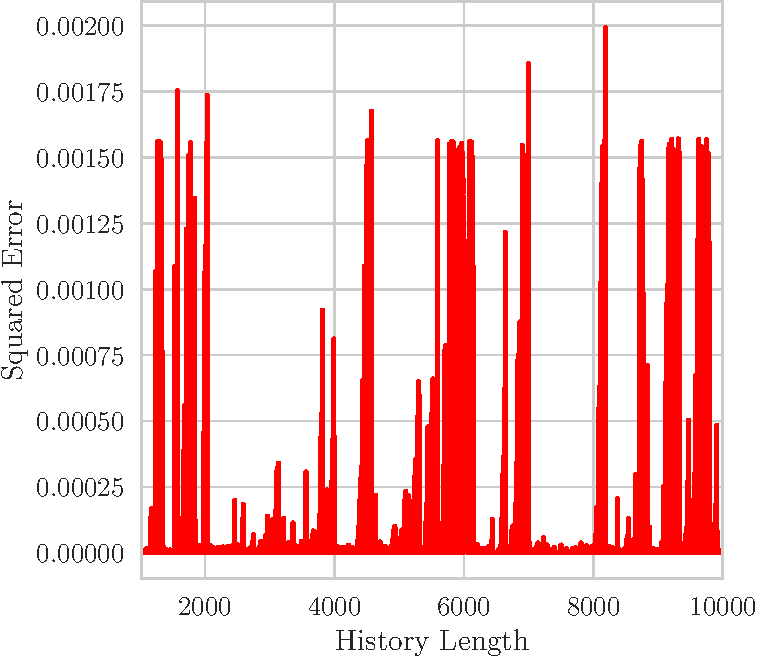
\includegraphics[scale=0.55]{figures/SE_trend_arima_10000.pdf}
        \caption{ARIMA on history upto past 10000}
    \end{subfigure}%
    ~ 
    \begin{subfigure}[h]{0.5\textwidth}
        \centering
        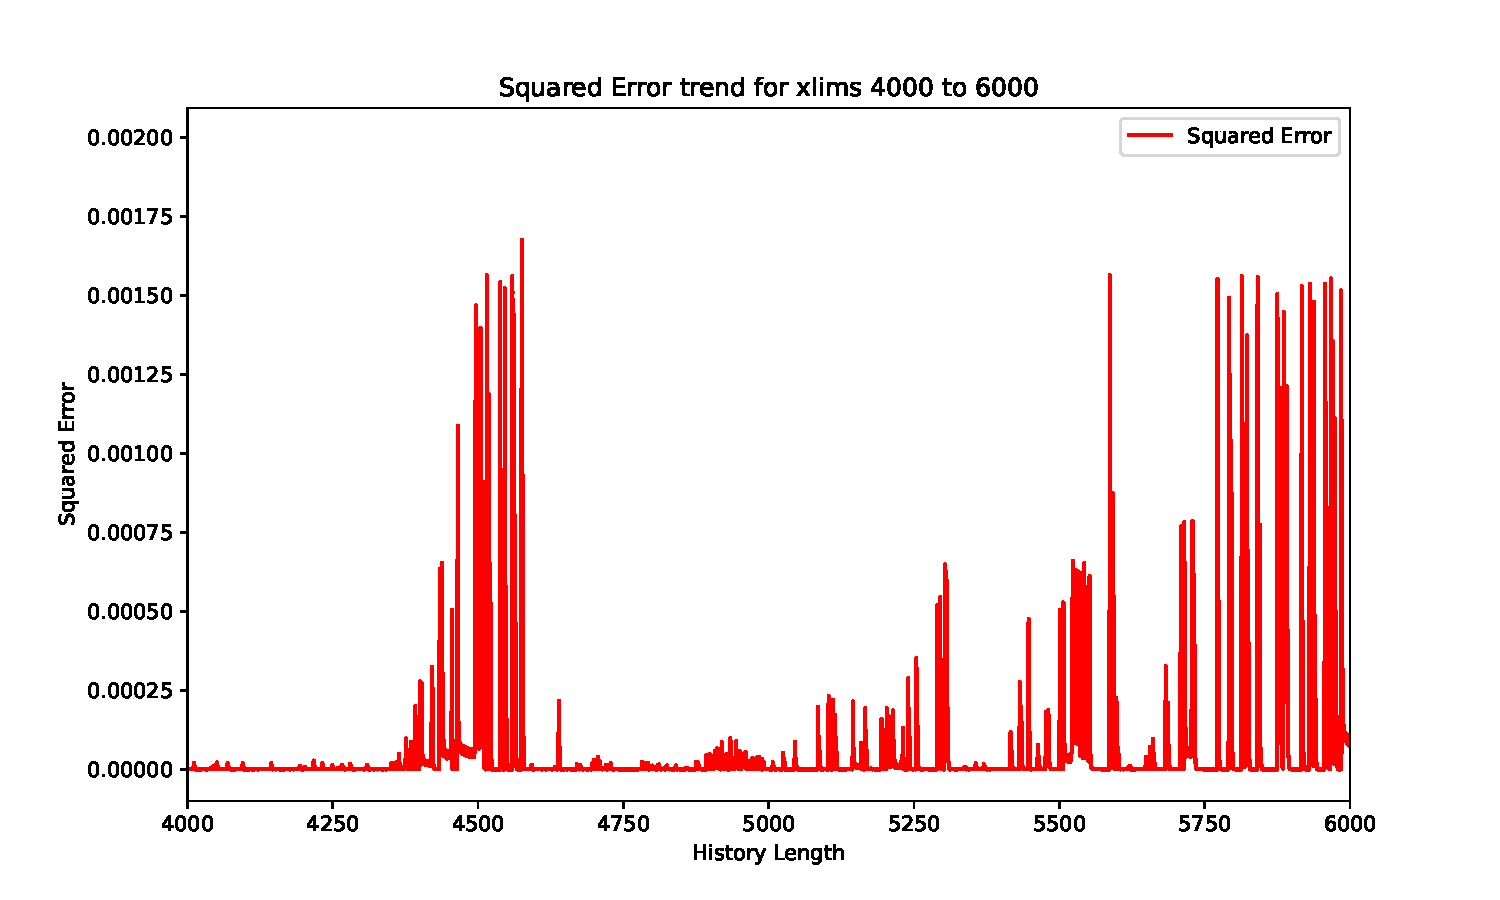
\includegraphics[scale=0.55]{figures/SE_trend_arima_30000.pdf}
        \caption{ARIMA on history upto past 30000}
    \end{subfigure}
    \caption{Squared error on the predictions of the ARIMA models trained to predict on a one-step rolling forecast }
    \label{fig:arima}
\end{figure*}

\paragraph*{Bi-Directional Long Short-Term Memory: }
Long Short-Term Memory (LSTM) memory networks\cite{lstm} have been the state-of-the-art models for sequence modelling for many years, before the introduction of the Transformer architecture. Prior to the same, LSTMs have successfully been used to successful solve several sequence-to-sequence tasks in NLP and time-series forecasting. Being a specialised RNN architecture, LSTMs suffer from the weaknesses of dependence on sequential processing and also vanishing gradients compared to the Transformer, as discussed in Section \ref{ssec:bgsequence}. However, in our project, it is is useful to include it as a baseline comparison, as it is a deep learning model designed to solve a very similar task. This in turn is helpful for us, in order to understand the learning behaviour of the Transformer to a greater extent.

We choose a Bi-Directional LSTM (Bi-LSTM)\cite{bilstm} architecture as a baseline, as it was the best known LSTM model for sequence tasks, prior to the use of Transformers becoming the norm for similar problems and present several variants of a trained Bi-LSTM model. In order to keep the comparison meaningful, we ensure that the total number of trainable parameters in the Bi-LSTM models, are similar to those in our NTT (${\sim}4M$ parameters). We only compare the pre-training task using the Bi-LSTM model, for our baseline. The pre-training process is the same as the NTT, we mask the \emph{last delay} in the in the input sequence of features, in the exact same manner in which we pre-train our initial NTT (as discussed in Section \ref{ssec:despatt}). The pre-training dataset is kept constant across all these models for uniformity in learning.

\begin{table}[htbp]
\centering
\begin{tabular}{ l   c   c  c }
\toprule
\emph{all values $\times10^{-3}$} & Pre-training by  \\
                                                       & {masking last delay}        \\
\midrule
\em{NTT}                                          &                \\
    \smallindent Standard                & 0.072           \\
     \noalign{\vskip 1mm}
\em{Bi-LSTM}                               &                \\
    \smallindent Aggregation + input embedding      & 0.062        \\
     \smallindent Aggregation + no input embedding     & 15.8        \\
     \smallindent No aggregation + no input embedding    & -       \\
     \smallindent  No aggregation + input embedding    & -       \\

\bottomrule

\end{tabular}
\caption{Mean Squared Error on pre-training NTT vs Bi-LSTM. The MSE is calculated on the predicted delay vs the actual delay value.}
\label{eval:table2}
\end{table}

The evaluation of pre-training Bi-LSTMs has been summarised in the Table \ref{eval:table2}. A-priori, we do not assume that the Bi-LSTM requires input data in a form equivalent to the NTT, in terms of aggregating our input features and passing the input features through an embedding layer before feeding it to the Bi-LSTM encoder layers. However, it is observed that the Bi-LSTM model learns efficiently and equally well as our NTT, only when we provide it the input data in the exact same method. The fact that it learns well under these conditions is not surprising at all, given that our aggregated sequences are not very long (limited to $48$ as of now). However the pre-training time for our NTT is much shorter (${\sim}12$ hours till convergence) as compared to pre-training the Bi-LSTM with the same input (${\sim}19$ hours till convergence) on identical hardware resources. We observe that if we do not use an embedding layer on the input to the Bi-LSTM, it performs poorly on the same pre-training objective, re-emphasising that such a learnable embedding is necessary to learn useful information from the features. Training the Bi-LSTM on non-aggregated input features (sequence size of $1024$) doesn't converge in practical time periods (a single epoch takes ${\sim}21$  hours to run on the same hardware) and hence, we do not evaluate those experiments further in our current scope.


\subsection{Evaluation on robust fine-tuning}
\label{ssec:robeval}

In the process of fine-tuning on our initial pre-trained NTT architecture, we showed that it generalised to predicting the \emph{last delay} value in a new environment, where the topology introduces $2$ bottlenecks using cross traffic (see Figure \ref{fig:topo_ft}). The fine-tuning data was much less than the pre-training data, and we argued that with generic enough pre-training, we could achieve extremely good performance on new datasets with relatively less amounts of fine-tuning. We now analyse this behaviour further and demonstrate the pre-training on a single bottleneck indeed helps in generalizing to topologies with multiple bottlenecks, in terms of requiring less data or less training effort or both. For these experiments, the pre-training process involves masking the delay value at the \emph{last position}.

For this, we generate a large amount of fine-tuning data, which is comparable in magnitude to the pre-training data (${\sim}1.2$ million packets). There is always, as a testing dataset, a constant subset of the fine-tuning dataset, which is unknown to and identical for every model variant. The NTT is now fine-tuned in multiple ways, we use the pre-trained NTT and fine-tune it on the entire fine-tuning dataset and separately on only $10\%$ of the fine-tuning dataset. Simultaneously, we also fine-tune the NTT with randomly initialised weights, both on the entire fine-tuning dataset and on only $10\%$ of the dataset. The $10\%$ subset of the fine-tuning data is the same across all variants. 

\begin{table}[htbp]
\centering
\begin{tabular}{ l   c   c  c }
\toprule
\emph{Model} &  MSE: Delay Prediction    & Layers Trained  & 	\# of Epochs Trained\\
			&		\emph{all values$\times10^{-3}$} 	&   	& \\ 
			

\midrule
\em{NTT}                                                               &                                             &   &  \\
    \smallindent Pre-trained  +   Fine-tune (full)                                  & 0.033                             & MLP Head only        & 5\\
    \smallindent Pre-trained  +   Fine-tune ($10\%$)                                  & 0.037                             & MLP Head only         & 9\\
    \smallindent From scratch  + Fine-tune (full)                                       & 0.036                             & Full NTT     & 13\\
     \smallindent From scratch  + Fine-tune ($10\%$)                                    & 0.118                             & Full NTT      &  15 \\
     \smallindent Pre-trained  +   No Fine-tune                                  & 0.108                             & -          & -\\
 
 \bottomrule

\end{tabular}
\caption{Comparing NTT across fine-tuning variants. The MSE is calculated on the predicted delay vs the actual delay value.}
\label{eval:table3}
\end{table}

The results on the fine-tuning variants are summarised in Table \ref{eval:table3}. From these experiments, it is evident that the initialising the NTT with \emph{pre-trained} weights helps the fine-tuning. With pre-training, using the entire fine-tuning dataset, we can reach a low MSE value in very few fine-tuning epochs (only $5$), whereas when we use only $10\%$ of the fine-tuning data, we can still reach similar values of MSE with just a few more epochs (only $9$). Also, with pre-training, it is only required to train the linear layers at the end of the NTT, which also reduces the training time on the whole. When we initialise \emph{from scratch}, we need much more effort to reach similar performance on the fine-tuning dataset. Using the entire fine-tuning dataset in this case, we achieve the same order of MSE, but only with training the entire NTT, for many more epochs. This behaviour is as expected as it is equivalent to performing pre-training on the fine-tuning dataset of approximately equal size. However, if we use only $10\%$ of the fine-tuning data in this case, we hardly learn anything which is seen in the MSE, as in this case, it is the same level of performance as initialising with pre-trained weights and not performing any fine-tuning. Based on these, we can effectively demonstrate that pre-training our NTT, does indeed help in a much quicker fine-tuning process \ie the NTT is able to generalise on learnt behaviour during pre-training, on tasks similar to the pre-training.


\subsection{Improved pre-training for NTT}
\label{ssec:impptt}

We also evaluate our NTT by pre-training it with different masking strategies. Concretely we no longer mask only the last packet delay in the sequence for pre-training and learning the sequence structure, but different positions in the sequence, as introduced in Section \ref{ssec:despatt}. The challenges and approaches to combining the masking of delays in the past, and the aggregation levels have already been discussed there; we now evaluate and compare the performance across these pre-training variants. The fine-tuning objectives haven't changed, we still use the same two fine-tuning environments, \emph{first} where we try to predict the delay of the last packet in the sequence data generated from the $2$ bottleneck topology and \emph{second} where we try to predict the MCT, based on the most recent packet data. Given the nature of the new pre-training, our primary expectation  is that the MCT prediction task should benefit from it. This is because for MCT prediction, we use the average pooled encoded state from the NTT's Transformer Encoder output stage and we expect the information contained in this ``average state'' to be higher with better, overall learning sequence structure, enabled by bi-directional pre-training. 

The final challenge is to decide on the frequency of masking packet delays across variable levels of packet aggregation \ie how often should one mask delays from non-aggregated packets and how often should one mask delays from aggregated packets. To handle this, we experiment with several masking strategies, in increasing order of complexity and number of elements masked at every step, and evaluate the performance in every case.
\begin{itemize}
\item \emph{Choose from last $16$:} We always mask one packet delay, by choosing uniformly over one element in the $16$ most recent packets. In this method, we never mask a delay from a packet which is aggregated.
\item \emph{Choose from last $32$:} We always mask one packet delay, by choosing uniformly over one element in the $32$ most recent packets. In this method, we also never mask a delay from a packet which is aggregated.
\item \emph{Choose from NTT encoded states:} We choose uniformly over all $48$ encoded states of the NTT's output. If the encoded state corresponds to a single non-aggregated packet, we mask that packet's delay value. If the encoded state corresponds to aggregated packets, we mask all packet delays aggregated to that given value. In this method, we do not distinguish between levels of aggregation.
\item \emph{Choose from aggregation levels:} We choose uniformly over all $3$ (non)aggregation levels. If we end up with a non-aggregated level, we mask $1$ delay uniformly chosen over the non-aggregated packet delays. If we end up with \emph{one level} of aggregation, we uniformly choose $1$ aggregated value and we mask all packet delays aggregated to the chosen encoded state. If we end up with \emph{two levels} of aggregation, we mask all the packet delays in the first half ($512$) of the sequence, which aggregate to the chosen encoded state.
\end{itemize}

\begin{table}[htbp]
\centering
\begin{tabular}{ l   c   c  c  c}
\toprule
\emph{all values $\times10^{-3}$} & Pre-training  & \multicolumn{3}{c}{Fine-tuning} \\
\cmidrule{3-5}
                                                       & {Delay}        & {Delay(on full)}  & {Delay(on 10\%)}                           & {log MCT} \\
\midrule
\em{NTT}                                              & 		 &			  & 						   &          \\
    \smallindent Last 16                                &    0.054            &  0.042  &        0.046                        &    64        \\
    \smallindent Last 32                                & 0.063         & 0.052                   &        0.057  		   &  55        \\
     \smallindent From encoded states        & 0.063          & 0.049              &   0.053             	  &   51        \\
     \smallindent From aggregation levels     & 0.087          & 0.053              &  0.057              & 61       \\

     \bottomrule

\end{tabular}
\caption{Mean Squared Error for all differently masked pre-trained NTT models and tasks. The MSE is calculated on the predicted vs the actual value.}
\label{eval:table4}
\end{table}

Referring to Table \ref{eval:table4}, we see that the different masking strategies do help learning structural information from the sequence of packet data better, especially for the MCT prediction task. If we compare with Table \ref{eval:table3}, we see a slight drop in performance when we fine-tune on the last position delay prediction, as opposed to the time when we pre-trained the NTT to predict the last delay too. This is expected behaviour as now the pre-training and fine-tuning tasks for delay prediction are not identical. If we compare with Table \ref{eval:table1}, we do see quite a bit of improvement in the MCT prediction. We evaluate the MCT prediction further and refer to Figure \ref{fig:mct_mask}. We see that with variable position masking, we reach lower levels of error with much fewer epochs of training in general, as opposed to when we have the masked pre-training only on the last delay position, which is enabled by the bi-directionality in the masked learning process. Given our current datasets, it is not possible to conclusively decide on ``one best" masking strategy for pre-training. However, we can definitively conclude that masking on variable position does help in better network dynamics learning from the sequence and in turn, better generalization, which is our ultimate goal.

\begin{figure*}[h]
    \centering
    \begin{subfigure}[h]{0.5\textwidth}
        \centering
        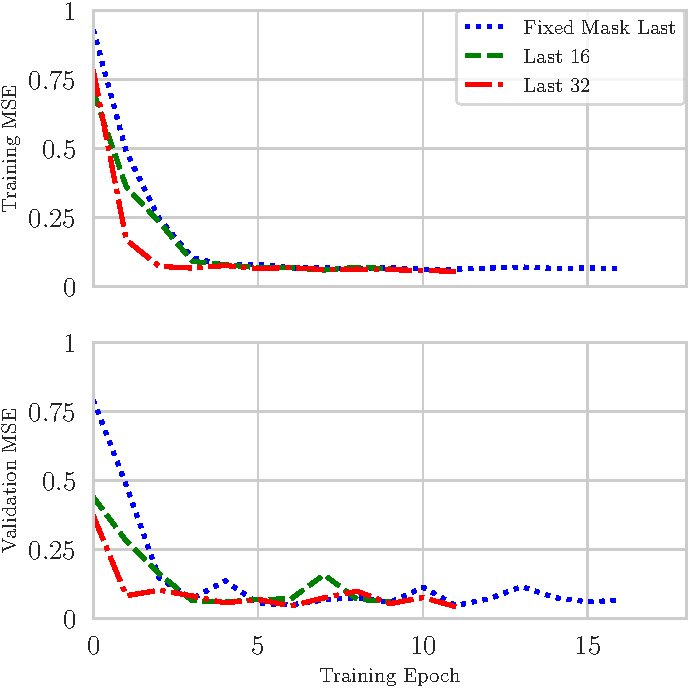
\includegraphics[scale=0.71]{figures/finetune_mct_loss_comparison.pdf}
        \caption{Pre-train with no mask over aggregated delays}
    \end{subfigure}%
    ~ 
    \begin{subfigure}[h]{0.5\textwidth}
        \centering
        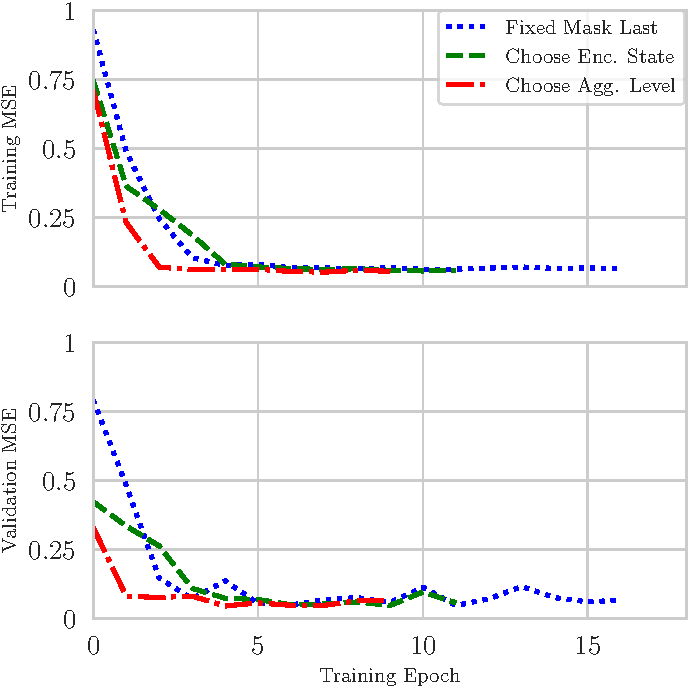
\includegraphics[scale=0.71]{figures/finetune_mct_loss_comparison_agg.pdf}
        \caption{Pre-train with also mask over aggregated delays}
    \end{subfigure}
    \caption{Mean-square error for prediction of message
time completion over different pre-training masks}
    \label{fig:mct_mask}
\end{figure*}

Finally, the NTT architecture for pre-training needs to be modified slightly, when we change the masking strategy for learning. For the cases of \emph{choosing from last $16$}, \emph{choosing from last $32$} or \emph{choosing from NTT encoded states}, we use the standard NTT model, with aggregation, followed by a Transformer encoder, followed by a set of linear layers. This method works well in all of the above cases, but does not work in the case of \emph{choosing from aggregation levels}. The most probable reason for this is, that due to equally choosing between the levels of aggregation, every $1/3^{rd}$ of the choices, a completely different type and number of delay values are masked. To handle this, we use three independent instances of the same set of linear layers, one for each kind of aggregation level, in order to effectively learn from each aggregation, and not have a single set of neurons ``pulled" in different directions for every type of masked value.\footnote{We move further studies on using multiple instances of linear layers to Appendix \ref{app:b}.}


\subsection{Evaluation on bigger topologies}
\label{ssec:comptop}

Till now, our experimental studies have been carried out on the single link topology as shown in Figure \ref{fig:topo_ft}. Our feature from the network state to learn the network dynamics is \emph{end-to-end delay}, which is the combination of the \emph{queuing delay} and the \emph{path delay}. As we had a single link topology for our evaluation, the \emph{path delay} was always constant and learning the dynamics was dominated by the queuing delay factor. We move to evaluation on a larger topology now, with different paths of multiple lengths, in order to also have more contribution from the path delay in our \emph{end-to-end delay} metric. Our method of traffic generation is similar to before, we have multiple applications sending traffic but we also have multiple receivers. We will always have cross-traffic as the data we generate is for fine-tuning.

We hypothesise that learning the network dynamics effectively from a single bottleneck, should be enough to generalise to similar dynamics on multiple bottlenecks , as shown in our new setup in Figure \ref {fig:topo_ft_big}, to a reasonable extent. Hence we will use our pre-trained NTT and fine-tune the model on the packet data generated in our new topology, and expect to generalise based on the prior learnt behaviour. For these experiments, we will use the NTT, which is pre-trained on masking the \emph{last delay}, as our objective is to explore the possibilities and ease of generalizing network dynamics to larger topologies, based on pre-training, rather than achieving the best possible results from it.

\begin{figure}[h]
  \begin{center}
    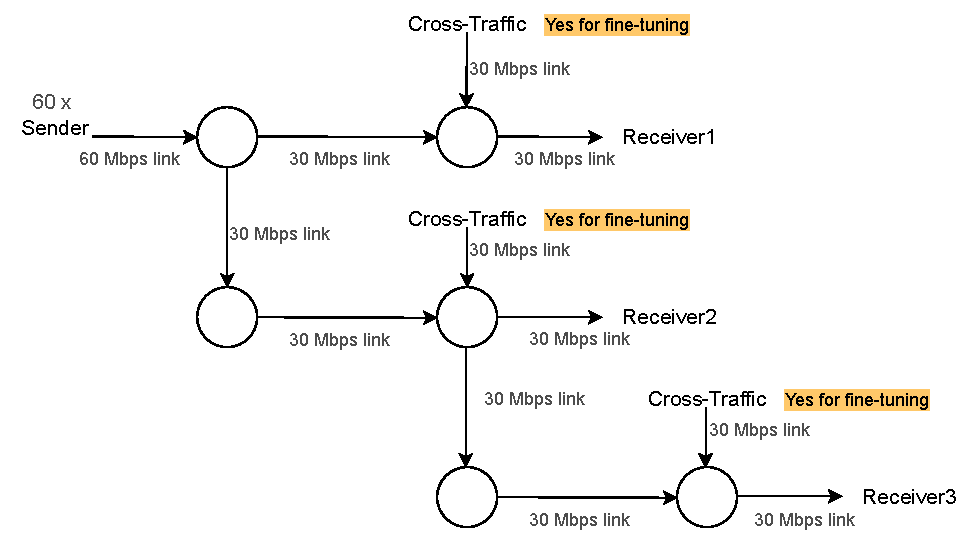
\includegraphics[scale=0.7]{figures/complex_topo.pdf}
    \caption{Fine-tuning data generation on larger topology}
    \label{fig:topo_ft_big}
  \end{center}
\end{figure}

Will add results here after the experiments are done, as they are not ready yet. Table will be similar  in layout to Table \ref{eval:table3}. The idea is to generate a new big dataset on the bigger topology (similar to original pre-training dataset size) and  compare fine-tuning with the whole and 10\% vs training the NTT from scratch on the whole and 10\% on this new dataset for delay prediction.



